\subsubsection{Hessian profiling analysis}
\label{sec:hessianprofiling}

To complement the results obtained
with the Bayesian reweighting approach,
we use a profiling method, suitable
for Hessian PDF sets, to estimate the effect of including
lattice-QCD pseudo-data into the fit~\cite{Paukkunen:2014zia,Camarda:2015zba}.
%
We
choose the HERAPDF2.0~\cite{Abramowicz:2015mha}
as a representative set of Hessian PDFs.
%
We consistently use the same lattice-QCD
pseudo-data on PDF moments to estimate the impact
on HERAPDF2.0 set, as in the case of the Bayesian reweighting
exercise presented in the previous section.
%
An additional advantage of the HERAPDF2.0 set is
the use
of a standard tolerance
$\Delta\chi^2=1$ for defining the 68\%-CL PDF
uncertainties, which ensures a
one-to-one correspondence between
the profiling and reweighting methods.

For Hessian PDF sets, the Hessian profiling method
can be used to both check the compatibility of new data with a given PDF set,
and also  estimate the impact these data will have on the PDFs. 
In the following we describe the essential components of the profiling method, 
and assume  that the  Hessian PDF set uses a tolerance of $\Delta\chi^2=1$, 
which corresponds to 68\%~CL uncertainties,
as is the case with HERAPDF2.0 set.\footnote{In this exercise
we consider only the {\it experimental} HERAPDF2.0
uncertainties, but not the {\it model} and {\it parametrization}
variations, which are not suited for profiling.}
%
The central values of the considered moments are obtained using the central PDFs and the corresponding
errors are calculated according to:
\begin{equation}
\delta\mathcal{F}_i = \frac{1}{2} \sqrt{\sum_{k}\left(\mathcal{F}_i(f_k^+)-\mathcal{F}_i(f_k^-)\right)^2}\, ,
\quad i=1,\ldots,N_{\rm mom} \, ,
\end{equation}
where $k$ labels the number of error PDFs (Hessian eigenvectors)
which have both a positive and negative direction.
%
In the profiling method, one considers a $\chi^2$ function in which the $\chi^2$ of the new
data has been added to the initial $\chi^2_0$, namely
\begin{equation}
\label{eq:newchi2}
\chi^2_{\text{new}} = \chi_0^2 + \sum_{k}^{N_{\text{eig}}} z_k^2
                    + \sum_{i=1}^{N_{\text{data}}}
                      \frac{\lp \mathcal{F}_i - \mathcal{F}_i^{\rm(exp)}\rp^2}
                           {\lp\delta\mathcal{F}_i^{\rm(exp)}\rp^2}\,,
\end{equation}
where $\chi^2_0$ is the value of the $\chi^2$ function in the minimum of the initial PDF set,
$z_k$ are the parameters diagonalizing the Hessian matrix of the initial PDF set,
$N_{\text{eig}}$ is the dimension of the eigenvector space in which initial Hessian errors are defined
(half of the number of error PDFs), $\mathcal{F}_i^{\rm(exp)}$ is the new
\hbox{(pseudo-)data},
and $\mathcal{F}_i$ the corresponding theory prediction.

In the spirit of the Hessian method, the new theory predictions $\mathcal{F}_i$ can be expanded
using a linear approximation:
\begin{equation}
\mathcal{F}_i \simeq \mathcal{F}_i[S_0] + \sum_k \frac{\partial\mathcal{F}_i[S]}{\partial z_k}\bigg|_{S=S_0} z_k \quad
              \simeq \mathcal{F}_i[S_0] + \sum_k D_{ik} w_k \ ,
\end{equation}
where $S_0$ represents the central PDF and we have defined
\be
D_{ik}=\frac{1}{2}(\mathcal{F}_i[S_k^+]-\mathcal{F}_i[S_k^-]) \, ;
\ee
here the  derivative has been approximated by a finite difference of the 
Hessian PDF error sets $S_k^{\pm}$.
%
The new $\chi^2$ of Eq.~\eqref{eq:newchi2} can now be minimised with respect to the parameters $w_k$,
which results in:
\begin{equation}
%\boldsymbol{\vec{w}_{\text{{\bf min}}}} = \boldsymbol{-B^{-1}} \boldsymbol{\vec{a}},
%
w_k^{min}  = \sum_n \ -B_{kn}^{-1} \, a_n \quad ,
\end{equation}
where we have introduced
\begin{equation}
%\begin{split}
B_{kn} = \sum_i \frac{D_{ik}D_{in}}{\lp\delta\mathcal{F}_i^{\rm(exp)}\rp^2} + \delta_{kn},
%\\
\qquad
\qquad
a_k = \sum_i \frac{D_{ik}(\mathcal{F}_i[S_0] - \mathcal{F}_i^{\rm(exp)})}{\lp\delta\mathcal{F}_i^{\rm(exp)}\rp^2} \, . 
%\end{split}
\end{equation}

The key result of the Hessian profiling method
is that now the components of the solution 
%$\boldsymbol{\vec{w}_{\text{{\bf min}}}}$ 
$w_k^{min}$
define a new set
of PDFs representing a global minimum after including the new data:
\begin{equation}
f_{\text{new}} = f_{S_0} + \sum_{k=1}^{N_{\text{eig}}} \frac{f_{S_k^+}-f_{S_k^-}}{2} w_k^{\text{min}} \ .
\end{equation}
At the same time 
%$\boldsymbol{\vec{w}_{\text{{\bf min}}}}$ 
$w_k^{min}$
also  defines  a penalty term 
\begin{equation}
P = \sum_{k=1}^{N_{\text{eig}}} \lp w_k^{\text{min}} \rp^2 \, ,
\end{equation}
which can be used to estimate whether the new data is consistent with the initial set of PDFs.
%
Specifically, a value of
the penalty term of $P\ll1$ means that the new data is consistent
with that included in the original fit.
%
Finally, a set of new error PDFs can be also defined; in this case the matrix $B_{kn}$ plays the role of
the Hessian matrix from which the PDF uncertainties
can be obtained. 

We​ ​performed​ ​this​ ​study​ ​using​ ​the​ ​xFitter​ ​program​ ​\cite{Alekhin:2014irh}​ ​and​ ​assuming​ ​the​ ​same​ ​three
scenarios​ ​for​ ​the​ ​lattice-QCD​ ​pseudo-data​ ​as​ ​in​ ​Tab.~\ref{tab:scenarios}.​ ​The​ ​results​ ​are​ ​shown​ ​in​ ​Tab.~\ref{tab:unpolmomentsProf},
where​ ​we​ ​tabulate​ ​the​ ​uncertainties​ ​of​ ​the​ ​input​ ​HERAPDF2.0​ ​PDF​ ​in​ ​column​ ​two​ ​and​ ​the
corresponding​ ​uncertainties​ ​for​ ​each​ ​scenario​ ​in​ ​columns​ ​three​ ​to​ ​five.​ ​Note​ ​that​ ​we​ ​list​ ​the
analogous​ ​results​ ​from​ ​the​ ​reweighting​ ​method,​ ​applied​ ​to​ ​the​ ​NNPDF​ ​3.1​ ​data​ ​set,​ ​in​ ​Tab.~\ref{tab:unpolmomentsrw}


%%%%%%%%%%%%%%%%%%%%%%%%%%%%%%%%%%%%%%%%%%%%%%%%%%%%%%%%
\begin{table}[h]
  \centering
  \renewcommand{\arraystretch}{1.3} 
\begin{tabular}{c||c|c|c|c}
  \hline &  Original  & Scen A  &  Scen B  &  Scen C  \\
  \hline
  \hline
  $\la x\ra_{u^+}$     &  $0.3720\pm 0.0036$  &  $0.3720\pm 0.0030$  &  $0.3720\pm 0.0027$  &  $0.3720\pm 0.0020$ \\
  $\la x\ra_{d^+}$     &  $0.1845\pm 0.0053$  &  $0.1845\pm 0.0028$  &  $0.1845\pm 0.0023$  &  $0.1845\pm 0.0015$ \\
  $\la x\ra_{s^+}$     &  $0.0346\pm 0.0037$  &  $0.0346\pm 0.0015$  &  $0.0346\pm 0.0012$  &  $0.0346\pm 0.0009$ \\
  $\la x\ra_{g}$       &  $0.4006\pm 0.0078$  &  $0.4006\pm 0.0042$  &  $0.4006\pm 0.0035$  &  $0.4006\pm 0.0024$ \\
  $\la x\ra_{u^+-d^+}$ &  $0.1875\pm 0.0074$  &  $0.1875\pm 0.0045$  &  $0.1875\pm 0.0039$  &  $0.1875\pm 0.0027$ \\
  \hline
\end{tabular}
\caption{\small Values of the unpolarised PDF moments
  used as lattice-QCD pseudo-data, as well as the corresponding results
  after the profiling  for the
three scenarios summarised in Tab.~\ref{tab:scenarios}.
%
The HERAPDF2.0 PDFs were used, and the PDF uncertainties quoted correspond in all cases to 68\%~CL intervals.
%
The corresponding results of applying the reweighting method
to NNPDF3.1 were listed in Tab.~\ref{tab:unpolmomentsrw}.
\label{tab:unpolmomentsProf}
}
\end{table}
%%%%%%%%%%%%%%%%%%%%%%%%%%%%%%%%%%%%%%%%%%%%%%%%%%%%%%%%

From a comparison of Tab.~\ref{tab:unpolmomentsProf} to Tab.~\ref{tab:unpolmomentsrw},
we observe a consistent trend compared with the reweighting of NNPDF3.1.
%
The relative reduction of the PDF uncertainties is larger
in this case though, for example, for $\la x\ra_{d^+}$ ( $\la x\ra_{s^+}$
and  $\la x\ra_g$) we find a reduction by a factor of roughly
four (four and three, respectively) compared to the original
HERAPDF2.0 uncertainties.
%
The constraining power of the lattice-QCD pseudo-data
on the PDF moments appears to be more significant in the
HERAPDF2.0 case than in the NNPDF3.1, because it includes only DIS data, while the latter
is a global fit containing a wider variety of
input data sets (and thus characterised by smaller
PDF uncertainties to begin with).

In Fig.~\ref{fig:pdfsProf} we present a
comparison of the
$u^+$, $d^+$, $g$, and $s^+$ PDFs at the scale of $Q^2=4$ GeV$^2$
between the original  HERAPDF2.0 set and the results of the profiling
exercise for scenarios A, B and C.
%
As mentioned above, only the {\it experimental} PDF uncertainties are shown
in this comparison,
but not the {\it model} and {\it parametrization} variations.
%
The corresponding results based on the reweighting
of NNPDF3.1 were shown in Figs.~\ref{fig:impactUnpol}
and~\ref{fig:impactUnpollargex}.

%%%%%%%%%%%%%%%%%%%%%%%%%%%%%%%%%%%%%%%%%%%%%%%%%%%%%%%%
\begin{figure}[!t]
\centering
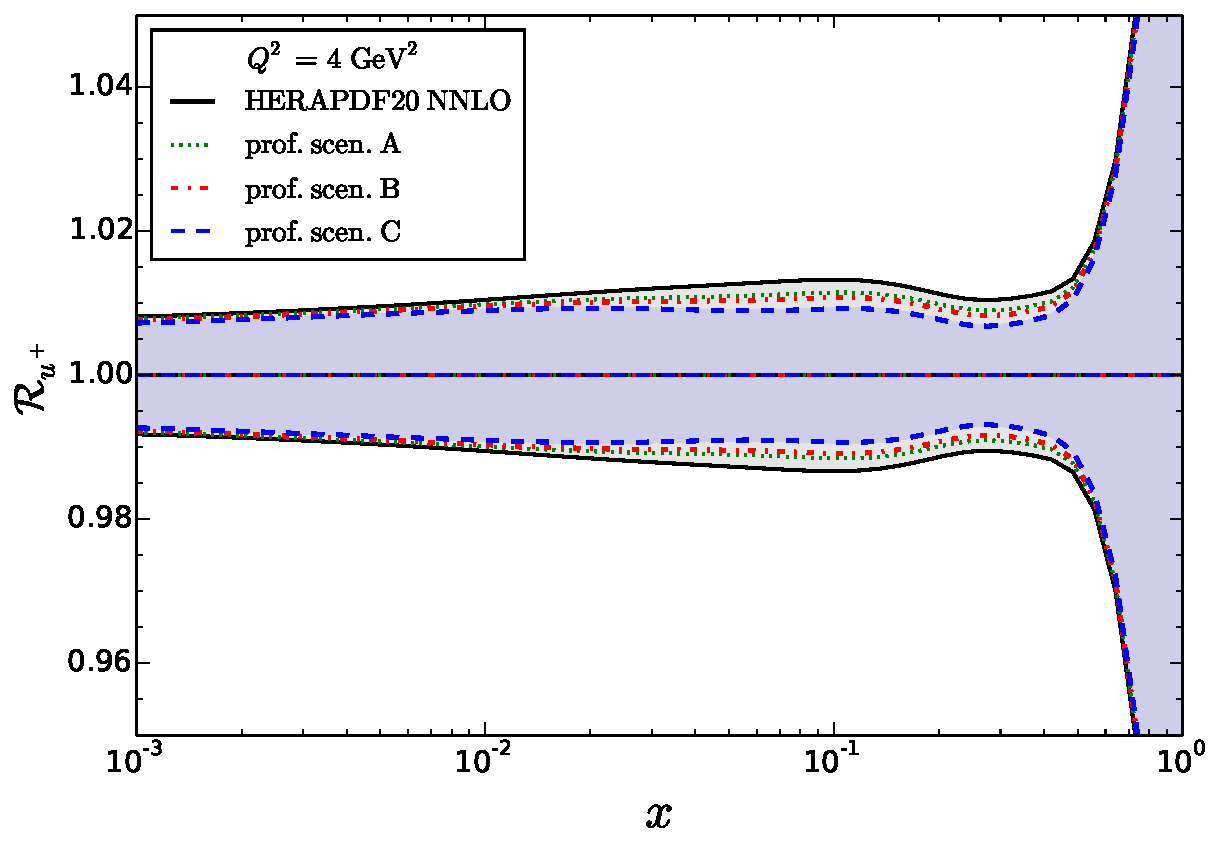
\includegraphics[width=0.45\textwidth]{plots/ratio_uPubar_Q2.pdf}
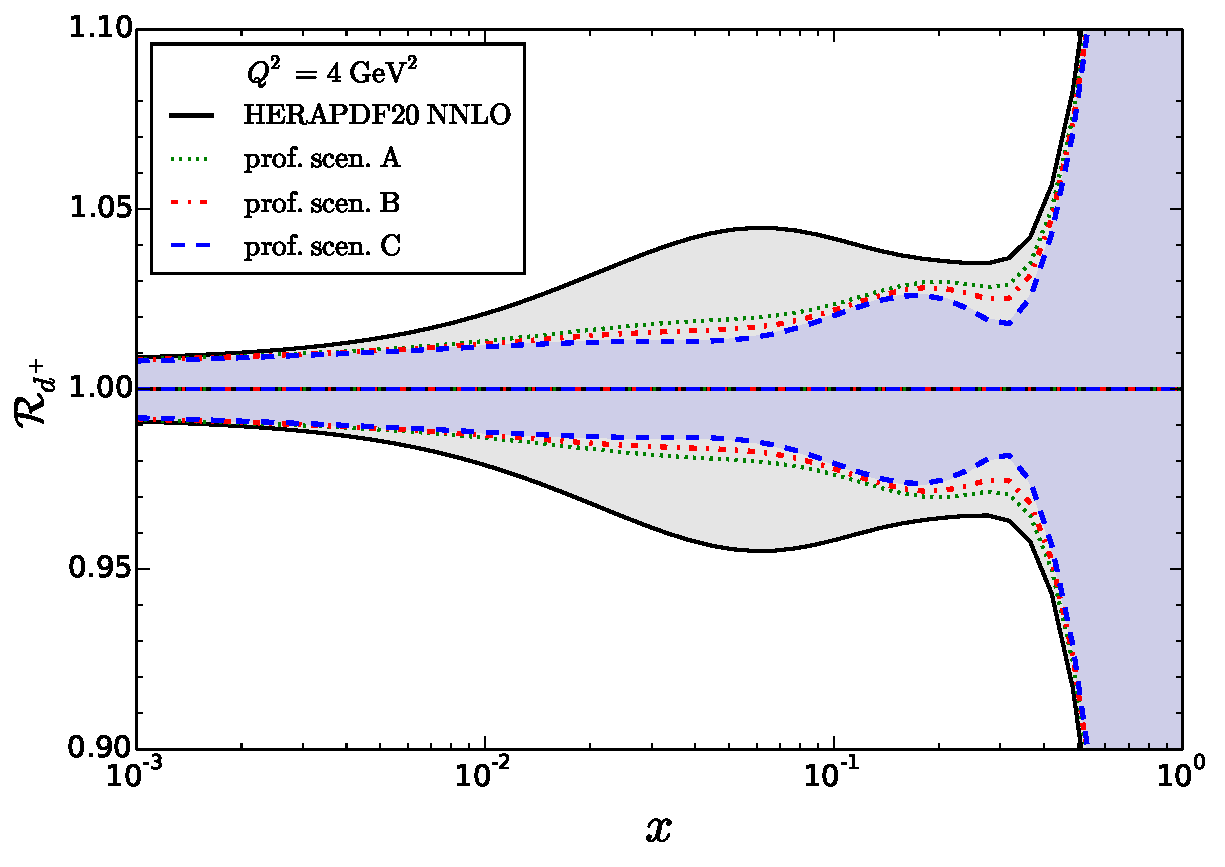
\includegraphics[width=0.45\textwidth]{plots/ratio_dPdbar_Q2.pdf}\\
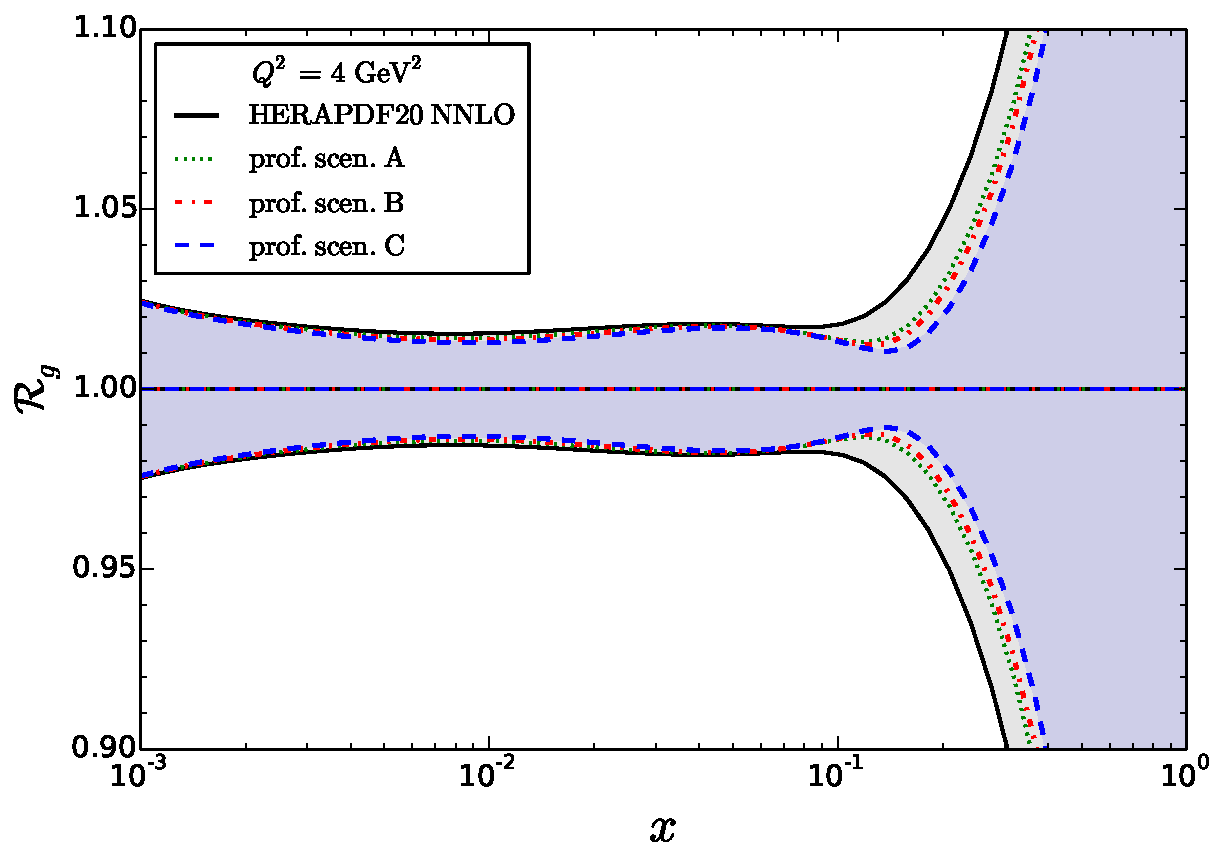
\includegraphics[width=0.45\textwidth]{plots/ratio_g_Q2.pdf}
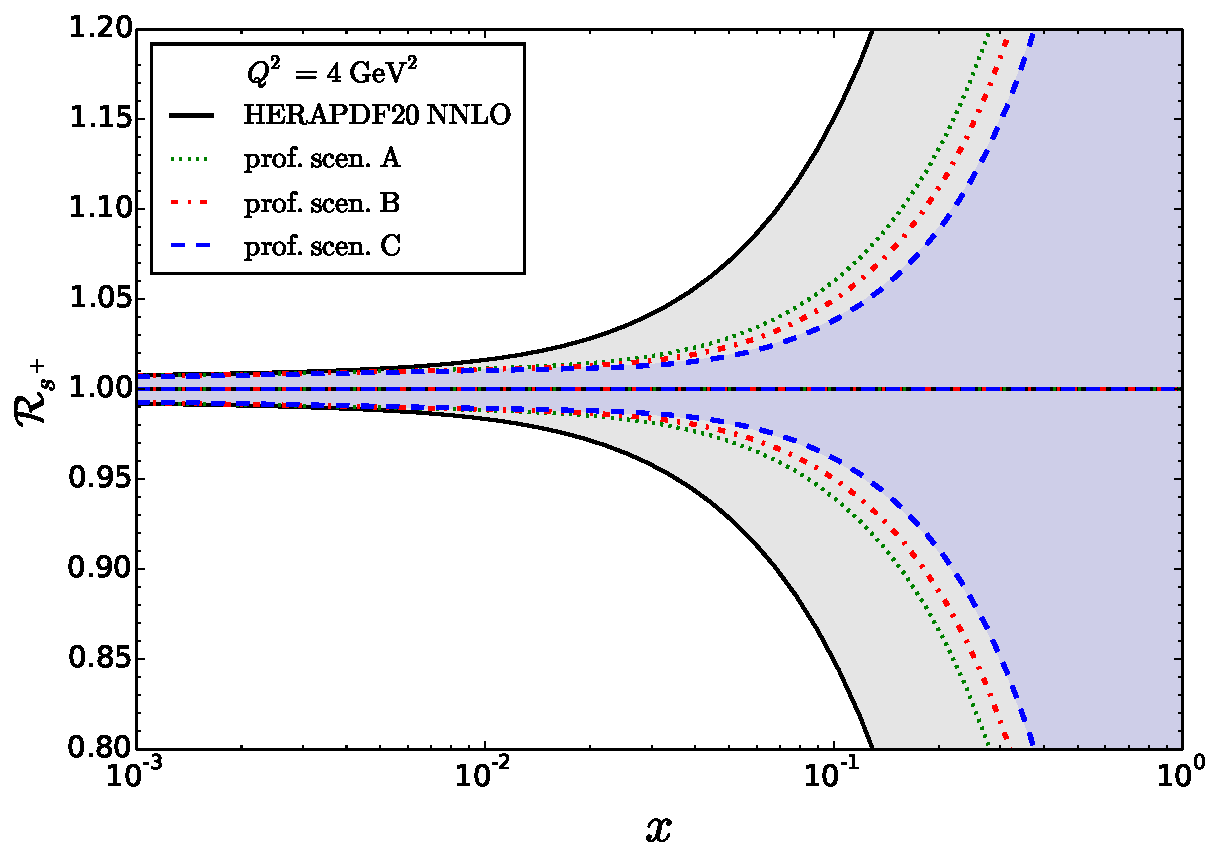
\includegraphics[width=0.45\textwidth]{plots/ratio_sPsbar_Q2.pdf}
\caption{\small Comparison
of the $u^+$, $d^+$, $g$, and $s^+$ PDFs at the scale of $Q^2=4$ GeV$^2$
between the original  HERAPDF2.0 set and the results of the profiling
exercise accounting for the constraints of
the lattice-QCD moments
pseudo-data in scenarios A, B and C.
%
Only the {\it experimental} PDF uncertainties are shown,
but not the {\it model} and {\it parametrization} variations.
}
\label{fig:pdfsProf}
\end{figure}
%%%%%%%%%%%%%%%%%%%%%%%%%%%%%%%%%%%%%%%%%%%%%%%%%%%%%%%%

From Fig.~\ref{fig:pdfsProf} we see that, as expected, the
impact of the lattice pseudo-data is greatest in the medium and large-$x$ regions.
%
The precise impact on the PDFs is rather
similar for the three scenarios, with the most optimistic
scenario C leading to the largest reduction in uncertainties.
%
The quark flavor combinations that are most affected by the
lattice-QCD pseudo-data are the $d^{+}$ and $s^{+}$ PDFs,
and, to a lesser extent, the gluon PDF.
%
The improvement in the PDF uncertainties for $d^{+}$ and $s^{+}$
occurs because the DIS data
used in HERAPDF2.0 includes only limited constraints
on quark flavour separation, ​and,​ ​for​ ​these​ ​PDFs,​ ​the​ ​lattice-QCD​ ​pseudo-data​ ​adds​ ​important​ ​new
information.
